\documentclass[a4paper,12pt]{article}

% Packages
\usepackage[nottoc,notlof,notlot]{tocbibind} 
\usepackage[margin=1in]{geometry}
\usepackage{changepage}
\usepackage{graphicx}
\usepackage{caption}
\usepackage{subcaption}
\usepackage{hyperref}
\usepackage{fancyhdr}
\usepackage{titletoc}
\usepackage [english]{babel}
\usepackage [autostyle, english = american]{csquotes}
\usepackage{lmodern}
\usepackage{sectsty}
\usepackage[font=small,labelfont=bf,font=normalfont]{caption}


% Page Style
\pagestyle{fancy}
\fancyhf{}
\fancyhead[L]{SRS Document}
\fancyhead[C]{}
\fancyhead[R]{Last revised: 10 August 2017}{\fontfamily{lmss}\selectfont}
\renewcommand{\headrulewidth}{0.4pt}
\fancyfoot[L]{Code 9}
\fancyfoot[C]{}
\fancyfoot[R]{Page \thepage}
\renewcommand{\footrulewidth}{0.4pt}

\sectionfont{\fontfamily{lmss}\selectfont}
\subsectionfont{\fontfamily{lmss}\selectfont}
\subsubsectionfont{\fontfamily{lmss}\selectfont}


% TOC levels
\setcounter{tocdepth}{5}
\setcounter{secnumdepth}{5}

\begin{document}\fontfamily{lmss}\selectfont
    \begin{center}\thispagestyle{empty}
    	\begin{figure}[h]
			\centering
			
\includegraphics[width=0.60\linewidth]{Graphics/uplogo.jpg}
	 	\end{figure}
    
        \newline
        {\Huge\fontfamily{lmss}\selectfont 
        Capstone 2017 \linebreak
        Project Management System \linebreak 
        \par}
        
        \begin{figure}[h]
			\centering
			
\includegraphics[width=0.3\linewidth]{Graphics/code9.png}
	    \end{figure} 
        
        \begin{LARGE}\fontfamily{lmss}\selectfont
            Seonin David
            \linebreak
            \linebreak
            Joshua Moodley
            \linebreak
            \linebreak
            Jacques Smulders
            \linebreak
            \linebreak
            Jordan Daubinet
            \linebreak
            \linebreak
            Nicaedin Suklul
        \end{LARGE}
    \end{center}
    
    \begin{figure}[b]
			\centering
			
\includegraphics[width=0.3\linewidth]{Graphics/kpmgLogo.jpg}
	\end{figure}  
    
    \newpage
    \tableofcontents
	\clearpage
    \newpage

\begin{table}[]
\centering
\label{my-label}
\resizebox{1.2\textwidth}{!}{%
\begin{tabular}{|l|l|}
\hline
Document Title          & Software Requirements Specification                                                                                                                                            \\ \hline
Document Identification & Document 0.0.2                                                                                                                                                                 \\ \hline
Author                  & \begin{tabular}[c]{@{}l@{}}Seonin David, Joshua Moodley, Jaques Smulders,\\  Jordan Daubinet, Nicaedin Suklul\end{tabular}                                                     \\ \hline
Version                 & 0.0.2                                                                                                                                                                          \\ \hline
Document Status         & \begin{tabular}[c]{@{}l@{}}Second Version - contains an updated non-functional requirements\\ section, as well as a new format for the Architectural Requirements\end{tabular} \\ \hline
\end{tabular}
}
\end{table}

\linebreak

\begin{table}[]
\centering
\label{my-label}
\resizebox{1.2\textwidth}{!}{%
\begin{tabular}{|llll|}
\hline
Version & Date         & Summary                                                                                                                                                & Authors                                                                                                                       \\ \hline
0.0.1   & 25 May 2017  & \begin{tabular}[c]{@{}l@{}}First draft contains functional\\ requirements, use case diagrams\\ and a deployment diagram\end{tabular}                   & \begin{tabular}[c]{@{}l@{}}Seonin David, Joshua Moodley, \\ Jaques Smulders, Jordan Daubinet, \\ Nicaedin Suklul\end{tabular} \\ \hline
0.0.2   & 21 June 2017 & \begin{tabular}[c]{@{}l@{}}Second draft contains an updated \\ structure for Architectural requirements\\ and non-functional requirements\end{tabular} & \begin{tabular}[c]{@{}l@{}}Seonin David, Joshua Moodley,\\  Jaques Smulders, Jordan Daubinet, \\ Nicaedin Suklul\end{tabular} \\ \hline
\end{tabular}
}
\end{table}

\clearpage
\section{Introduction}
    \subsection{Purpose}
      \begin{flushleft}
        The purpose of this document is to provide a detailed description of the requirements for the Project Management System. It will explain the purpose and features of the system, as well as system constraints. This document is intended to be proposed to University of Pretoria lecturers and the KPMG the project owner, as well as a reference for developing the first version of the project management system.
      \end{flushleft}
 
  \subsection{Scope}
      \begin{flushleft}
        KPMG currently have a web based project management system named EMS which handles allocation and management of assigned projects for all employees and project managers.The current system does not cover the spectrum of requirements that they demand. They require further functionality from the system and they wish to control more business needs and communication through a single portal. The client needs require us to create a new design of their current system and an update of their current interface.
        \linebreak
        \linebreak
        KPMG's project management system will be a web based application that allows for the creation and management of projects. It will handle a notification system for notification requests and notification acknowledgements and and per-user calendar overview to display all current project information currently assigned to that user. For all projects currently administered, the system is also required to display client Location and direction information to the employees assigned to the project.
        \linebreak
        \linebreak
        KPMG's project management system will further require Microsoft Outlook integration in the form of a toolbar to be created for Microsoft Outlook which manages the chain of responsibility for notification requests and notification acknowledgements.
      \end{flushleft}
      
    \subsection{Assumptions and Dependencies}
      \begin{itemize}
          \item \# :  number
          \item FR# : Functional Requirement #
          \item DB : Database
          \item ms : Milliseconds 
      \end{itemize} 
      
      \newpage
	\section{Architectural Requirements}
		\begin{adjustwidth}{2.5em}{0pt}
			%\addcontentsline{toc}{subsection}{\protect\numberline{}Introduction}
			\subsection{Introduction}
			\begin{flushleft}
				The system design to be implemented will be referred to as a Hybrid-tier System. This hybrid model is based off the n-tier (multi-layered) architecture, where the system is divided into layers. This multi-layered system is also referred to as a Client-Sever architecture. For this architecture, there are four tiers/layers. Those being: 
				\begin{enumerate}
					\item Presentation Tier
					\item Server Tier
					\item Database Tier
					\item AI (Artificial Intelligence) Algorithm Tier
				\end{enumerate}
				 Each layer will be modifiable without needing to change the entire application. As a result of the aforementioned, maintenance and adding extra functionality is easier. Overall complexity of code over all layers will be reduced, thus making the layers reusable in other applications. Since the layers do not act like a traditional n-tier where one would delegate tasks to other layers; once a request goes to the server tier, the server will decide if it will go to the database tier or the AI tier which then goes to the database tier. Thus showing an optimised parallel system to deal with requests.
				 Additionally, the use of this architecture system will allow different members of our team to modify separate layers without interference. It is possible to deploy each layer (specifically the database and server layers) over multiple locations for better reliability and performance. What differentiates the hybrid architecture from a traditional n-tier or client-server, is in how the layers are implemented. Figure \ref{fig:Deployment} shows the overall architecture of this hybrid system.
				 	\begin{figure}[h]
					 	\centering
				    	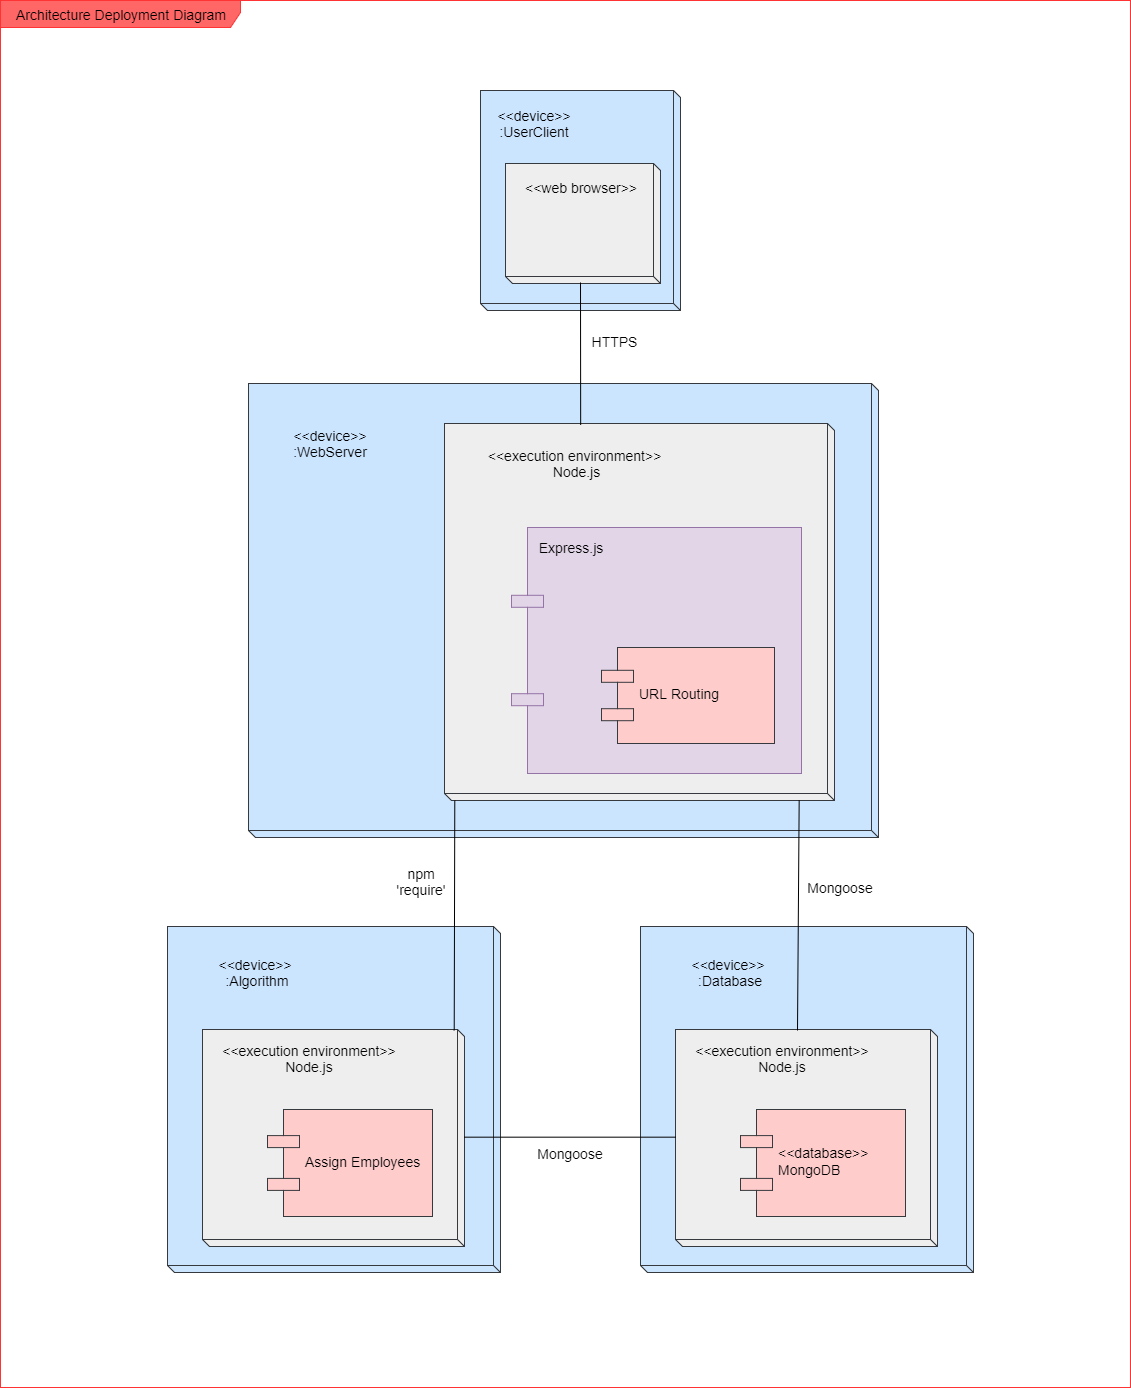
\includegraphics[width=0.5\linewidth]{Diagrams/deployment.png}
					 	\caption{Deployment Diagram: Hybrid-Tier Architecture}
					 	\label{fig:Deployment}
				 	\end{figure}
			\end{flushleft}
		
			%\addcontentsline{toc}{subsection}{\protect\numberline{}Presentation Tier}
			\subsection{Presentation Tier}
			\begin{flushleft}
			This is the layer the user will be interacting with. It encompasses the actual applications that can be developed (Android, iOS and web), and any interactions that the users may have with them. In this system, the user will primarily work with a web application as the front-end.
			\newline 
			
			\textbf{The presentation tier includes:}
			\begin{itemize}
				\item Displaying the user interface (UI), which the user will interact with. 
				\item Adding notification, forms, buttons and pages. 
				\item Providing an interface to trigger requests to the system. 
				\item Ultimately serving as a communication medium between pages on the front-end, and to send and receive data between the back-end.
			\end{itemize}
			\end{flushleft}
	
			%\addcontentsline{toc}{subsection}{\protect\numberline{}Server Tier}
			\subsection{Server Tier}
			\begin{flushleft}
			The server layer implements the business logic, and process all requests made by the front-end - it makes logical decisions based on the interactions from the presentation layer and then decides what or where data needs to go; either to the database layer or the AI layer.
			\newline
			
			\textbf{The server tier is responsible for:}
			\begin{itemize}
				\item Allow admin users to be able to add/remove/edit client projects, and assign employees to specific projects.
				\item Automatically update calendars of employees.
				\item Crosscheck projects before assigning them to an employee.
				\item Server communication over the internet.
				\item Scheduling Assistant calculations. 
				\item Limit an employee from being able to edit projects they have been assigned to.
				\item Allow an employee to add other events to his/her calendar if these do not clash with the pre-populated events.
				\item Session management.
			\end{itemize}
			\end{flushleft}
			
			\newpage
			%\addcontentsline{toc}{subsection}{\protect\numberline{}Database Tier}
			\subsection{Database Tier}
			\begin{flushleft}
				The data layer is where the information used by the presentation layer for sending and retrieving, is stored. This layer consists of:
				\begin{itemize}
					\item Recommended time slots where all employees are available. 
					\item Server storage with MongoDB
					\item View individual employee calendar and assigned projects. 
				\end{itemize}
			\end{flushleft}
		
			
			%\addcontentsline{toc}{subsection}{\protect\numberline{}AI (Artificial Intelligence) Algorithm Tier}
			\subsection{AI (Artificial Intelligence) Algorithm Tier}
			\begin{flushleft}
			    The AI layer houses the resource allocation algorithm, and is used by the server layer to allocate employees to a project. This layer runs off its own independent resources, and is dependent only on the database tier from which it retrieves resources necessary for the allocation algorithm.
			  
			\end{flushleft}
	\end{adjustwidth}
	
\section{Specific Requirements}
	\subsection{Functional Requirements}
		\subsubsection{FR1: Employee Functions}
			\begin{itemize}
				\item \textbf{FR1.1}: An employee will be able to log in to their account on the system
				\item \textbf{FR1.2}: An employee will be able to create their own profile with their        respective skills and previous work experience
				\item \textbf{FR1.3}: An employees will receive a notification when they are assigned to a    newly created project 
				
				\item \textbf{FR1.4}: An Employee must be able to to view their currently assigned           project and view their past completed projects that where assigned        to them on their profile. 
				
				\item \textbf{FR1.5}: An employee will be able to add personal or other events to the        calendar their calender, that do not clash with any existing               projects they are currently assigned to. If a newly created event        does clash, an error will be displayed.  
				
				\item \textbf{FR1.6}: When an employee clicks on a project in the calendar, it will show     all the project details and a map of the clients location should be       displayed as well as directions to the client.
				
				\item \textbf{FR1.7}: An employees will not be able to remove a project that is assigned     to them from their calender.
				
				\item \textbf{FR1.8}: Employees should confirm whether they have attended training or not, this will be conformed with trainer.
			\end{itemize}
	
	\subsubsection{FR2: Manager functions}
	\begin{itemize}
		\item \textbf{FR2.1}: A manager will be able to log in and create a project.
		
		\item \textbf{FR2.2}: A manager will be able to assign system recommended employees to a      newly created projects
		
		\item \textbf{FR2.3}: A manager will be able change employees if the manager is unhappy with     the recommendation by the system, pending director approval.
		
		\item \textbf{FR2.4}: A manager will be allowed to remove a project from the system, pending director approval
		
		\item \textbf{FR2.5}: A project manager will be able to view all projects that they are managing
	\end{itemize}
	
	\subsubsection{FR3: System Functions}
	\begin{itemize}
		\item \textbf{FR3.1}: The system will assign employees to a project based
		on their skill level and past project experience. 
		
		\item \textbf{FR3.2}: The system will find all the employees that have the required skills     for the job and give it to the manager as a recommendation.
		
		\item \textbf{FR3.3}: The system will only select employees if they are not already           assigned to a project.
		
		\item \textbf{FR3.4}: Employee data with skills and past work experience
		will be entered on the system and updated after each project. 
		
		\item \textbf{FR3.5}: System will reassign another employee, pending 
		approval, if an employee takes leave during the project.
		
		\item \textbf{FR3.6}: Every employee that is assigned to a project will get
		the full project duration and details on their calendar. 
		
		\item \textbf{FR3.7}: The system should be able to provide the location of and direction      to the client to all employees assigned to the respective project
		
		\item \textbf{FR3.8}:The system will preload all employees training dates
		at the beginning of the year. 
		
		
		\item \textbf{FR3.9}: The system will preload all employees training dates at the beginning of the year.
	\end{itemize}
	

\subsection{Non Functional Requirements}
 \subsubsection{Performance requirements}
    \subsubsubsection{Reasons for performance as a non-functional requirement}
    \begin{itemize}
        \item Performance is one of the core components of what is required from the project management system, it needs to be effective and efficient.
        
        \item Performance can play a large role in usability, usability describes the users experience well using the product. The project management system must deliver a positive user experience. 
    \end{itemize}
    
    \subsubsubsection{Strategies to achieve this non-functional requirement}
    \begin{itemize}
        \item The system needs to be able encompass over 200 concurrent connections.
        
        \item The DB needs to handle over 1000 requests and responses each second.
        
        \item The latency associated with verifying a users log in credentials must be fall under 200ms. 
        
        \item The latency associated with requesting and receiving a response for an accessible web page must fall under 50ms.
    \end{itemize}
    \subsubsubsection{Patterns to achieve these strategies}
    \begin{itemize}
        \item Expert Pattern
        \item Layer pattern
    \end{itemize}
    
    \begin{flushleft}
    The Expert pattern can be used to direct requests to different locations. The pattern ensures your program utilizes efficient resource management by directing requests and responses to the respectful parts of the system that can Handel them correctly. This relieves bottle necking a single part of the system with all responsibilities.
    \linebreak
    Utilizing the layer pattern allows us to divide our system into subsystems which can be run in separate locations.We can divide our initial system into A front end, a back end and a database manager. By splitting our system up, we can alter how many resources we allocate to each system, thus we utilize our recourse's efficiently and provide loose coupling between the different parts of the system. 
    \linebreak
    By combining the expert and layer pattern, we can handle different requests efficiently and correctly with their associated subsystem. 
    \end{flushleft}

\subsubsection{Quality requirements}
    \subsubsubsection{Reasons for quality as a non-functional requirement}
    \begin{itemize}
        \item By stating Quality requirements, you define the desired attributes which your program must have. Defining your programs attributes moulds key factors of its development and sets quality milestones and goals.  
        
        \item When the project is ready for deployment, the quality requirements which were set at the begging of development define how reliable the end product is or should be.
    \end{itemize}
    
    \subsubsubsection{Strategies to achieve this non-functional requirement}
    \begin{itemize}
        \item When Queried to allocate a team, the resource allocation algorithm must produce one within a maximum of 10 seconds.
        
        \item The system shall be available 99\% of the time, only going down in the duration of maintenance or while implementing updates.
        
        \item When queried for a project team and members are available, the resource allocation algorithm should never respond with no allocated team members. 
        
        \item When queried for a project team by a project manager, the resource allocation algorithm should provide a compatible and satisfactory project team to the project manager 85\% of queries made. 
    \end{itemize}
    
    \subsubsubsection{Patterns to achieve these strategies}
    \begin{itemize}
        \item This will depend on the pattern used by the artificial intelligence resource allocation algorithm. 
        \item layer
    \end{itemize}
    Using the layer pattern we can divide the responsibilities of quality to the respective three layers. Each layer handles its own quality management, this promotes loose coupling regarding quality dependencies between subsystems. Improvements can be made to separate layers independently to satisfy the systems quality requirements.
    
\subsubsection{Security requirements}
    \subsubsubsection{Reasons for Security as a non-functional requirement}
    \begin{itemize}
        \item Kpmg offers services in both data analysis and auditing. Both areas deal with highly confidential client information and regard security as top priority. The project management system may not have anything to do with these services, however it is a representation of kpmg's ethics and it must value security regarding client information with the same importance.
        
        \item If the project management system is to be hosted from the same physical servers as other company systems, it must have no area for exploitation. Security requirements ensures this.
        
        \item confidential information regarding projects should have no opportunities to be exploited to the public via malicious attacks on the system, security requirements protect the system from letting this happen.  
    \end{itemize}
    
    \subsubsubsection{Strategies to achieve this non-functional requirement}
    \begin{itemize}
        \item There is a hierarchy of users for the application. The range includes administrators, directors, project managers and further employees below these roles. Each user has different responsibilities and authority over the project which gives them project management options to govern the project that are not available to other users. Access to options available to users with a certain role should only be available to these users, session and verification management of the system will ensure this.
        
        \item 
    \end{itemize}
    
    \subsubsubsection{Patterns to achieve these strategies}
    \begin{itemize}
    \item Chain of responsibility
    \end{itemize}
    
    Using the chain of responsibility pattern, we can create a chain of handlers for our requests and responses. The client can send a request to the server which either handles the request or sends it to the database manager whereby the response is then sent back up the chain. This allows us to have greater control over the security of the system as a whole by carefully checking and handling each request at different stages before it can access any information from the database.
    
\subsubsection{Interface requirements}
    \subsubsubsection{Reasons for Interface as a non-functional requirement}
    \begin{itemize}
        \item Interface requirements cover a broad spectrum including the usability of the system as well as its hardware and software interfaces and their respective capabilities. 
        
        \item The usability of the system defines the user experience well using the system. To elicit a positive experience, the system must take into account and deploy many usability guidelines. KPMG wish to update their current project management system with a new design due to the lack of usability effectiveness of the current system. 
        
    \end{itemize}
    
    \subsubsubsection{Strategies to achieve this non-functional requirement}
    \begin{itemize}
        \item The new system's front should be developed with usability as its key target. its interface should have a modern and intuitive design which brings about a positive experience to the user using it.
        
        \item All subsystems should communicate with one another through http Get and Post requests.
    \end{itemize}
    
    \subsubsubsection{Patterns to achieve these strategies}
    \begin{itemize}
    \item layered pattern
    \end{itemize}
	
\subsection{Architecture Design}
\begin{paragraph}
        The system will be designed using the 3-tier architecture. The system is divided into three layers forming a presentation tier web application, a logic tier Node.js server and a data tier mongoDB database manager.
        \begin{itemize}
            \item 1. Presentation Layer
            \item 2. Logic Layer
            \item 3. Data Layer
        \end{itemize}
         Each layer will be modifiable without having to change the entire application. As a result of the aforementioned, maintenance and adding extra functionality is easier. Overall complexity of code over all layers will be reduced thus making the layers reusable in other applications.By using this architecture system will allow the different members in our teams to modify different layers without interference. It is possible to deploy each layer, specifically the data and server layers, over multiple different locations for better reliability and performance.
\end{paragraph}
 
  \subsubsection{Presentation Layer}
    \begin{paragraph}
       This is the layer the user interacts with, it encompasses the different front-end applications, and any interactions that the users have with them.     
    \end{paragraph}
    \textbf{The presentation layer include:  }
      \begin{itemize}
        \item What to display and when to display it, it’s the logic behind the web pages and the control between access from one to another.
      \end{itemize}
  
  \subsubsection{logic Layer}
    \begin{paragraph}
        The server layer contains all the business logic of the system - it makes logical decisions based on the interactions from the presentation above and the data layer below.   
    \end{paragraph}

    \textbf{The decisions made by this layer include:}
          \begin{itemize}
            \item Allow admin users to be able to add/ remove client projects and assign these to employees who will be working on these projects.
            \item Automatically update calendars of the employees.
            \item Crosscheck projects before assigning projects to an employee.
            \item Server communication over the internet.
            \item Scheduling Assistant calculations. 
            \item Limit an employee from being able to edit the projects that have been prepopulated.
            \item Allow an employee  to add other events to his/ her calendar if these do not clash with the prepopulated events.
            \item Session management.
          \end{itemize}
  
  \subsubsection{Data Layer}
    \textbf{The data layer is where the data and information used by the application layer is stored. This information includes:}
    \begin{itemize}
        \item Recommended time slots where all employees are available. 
        \item Server storage with mongodb
        \item View individual employee calendar and assigned projects. 
    \end{itemize}
    
\subsection{Architecture Constraints}
	\begin{itemize}
		\item The project must be completed in the given time frame with progress on        track with demo expectations.
		\item The project must not utilize technologies with require cost resources.
		\item The project must utilize Microsoft Outlook as a communication interface       for sending and confirming requests
		\item The project must be run as a local host and not deployed on a company         server
	\end{itemize}
    
\section{Use Case Diagrams}
	\subsection{Assigning Projects}
	\centering
	\includegraphics[width=15cm,height=15cm]{Functional_Use_Cases/Assigning_Projects.jpg}
	\subsection{Managing Projects}
	\includegraphics[width=15cm,height=15cm]{Functional_Use_Cases/Managing_Projects.jpg}
	\subsection{View Projects}
	\includegraphics[width=15cm,height=15cm]{Functional_Use_Cases/View_Projects.jpg}
	\subsection{Training}
	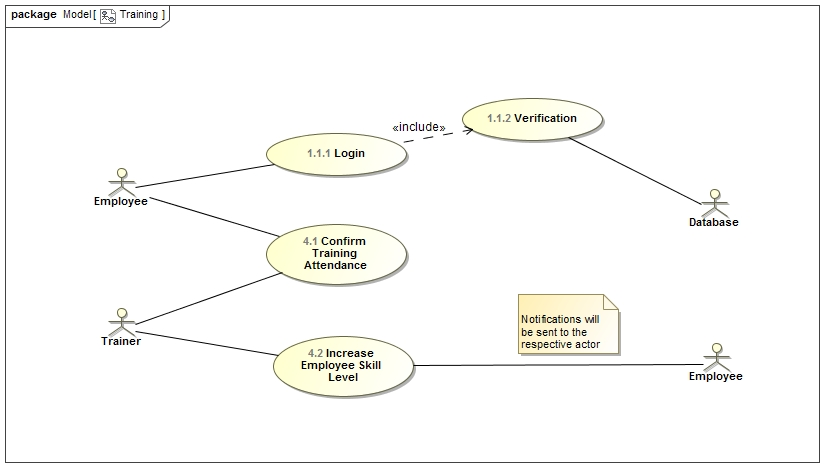
\includegraphics[width=15cm,height=15cm]{Functional_Use_Cases/Training.jpg}
	
\section{Deployment Diagram}
\includegraphics[width=15cm,height=15cm]{Functional_Use_Cases/KPMG.jpg}

\newpage

\section{Tracibility Matrix}
\begin{table}[]
\centering
\caption{Tracibility Matrix}
\label{my-label}
\resizebox{1.2\textwidth}{!}{%
\begin{tabular}{|l|c|c|c|c|c|c|c|c|c|c|c|c|c|c|c|c|}
\hline
       & \multicolumn{1}{l|}{Priority} & \multicolumn{1}{l|}{UC 1.1} & \multicolumn{1}{l|}{UC 1.2} & \multicolumn{1}{l|}{UC 1.3} & \multicolumn{1}{l|}{UC 1.4} & \multicolumn{1}{l|}{UC 1.5} & \multicolumn{1}{l|}{UC 2.1} & \multicolumn{1}{l|}{UC 2.2} & \multicolumn{1}{l|}{UC 2.3} & \multicolumn{1}{l|}{UC 2.4} & \multicolumn{1}{l|}{UC 3.1} & \multicolumn{1}{l|}{UC 3.2} & \multicolumn{1}{l|}{UC 3.3} & \multicolumn{1}{l|}{UC 3.4} & \multicolumn{1}{l|}{UC 4.1} & \multicolumn{1}{l|}{UC 4.2} \\ \hline
FR 1   &                               &                             &                             &                             &                             &                             &                             &                             &                             &                             &                             &                             &                             &                             &                             &                             \\ \hline
FR 1.1 & 2                             & X                           &                             &                             &                             &                             &                             &                             &                             &                             &                             &                             &                             &                             &                             &                             \\
FR 1.2 & 1                             &                             &                             &                             &                             &                             &                             &                             &                             &                             & X                           &                             &                             &                             &                             &                             \\
FR 1.4 & 3                             &                             &                             &                             &                             &                             &                             &                             &                             &                             &                             & X                           &                             &                             &                             &                             \\ \hline
FR 2   &                               &                             &                             &                             &                             &                             &                             &                             &                             &                             &                             &                             &                             &                             &                             &                             \\ \hline
FR 2.1 & 2                             & X                           &                             &                             &                             &                             &                             &                             &                             &                             &                             &                             &                             &                             &                             &                             \\
FR 2.2 & 3                             &                             & X                           &                             &                             &                             &                             &                             &                             &                             &                             &                             &                             &                             &                             &                             \\
FR 2.3 & 1                             &                             &                             &                             &                             &                             &                             & X                           &                             &                             &                             &                             &                             &                             &                             &                             \\ \hline
FR 3   &                               &                             &                             &                             &                             &                             &                             &                             &                             &                             &                             &                             &                             &                             &                             &                             \\ \hline
FR 3.1 & 4                             &                             &                             &                             & X                           &                             &                             &                             &                             &                             &                             &                             &                             &                             &                             &                             \\
FR 3.2 & 1                             &                             &                             & X                           &                             &                             &                             &                             &                             &                             &                             &                             & X                           &                             &                             &                             \\
FR 3.3 & 5                             &                             &                             & X                           &                             &                             &                             &                             &                             &                             &                             &                             & X                           &                             &                             &                             \\
FR 3.4 & 6                             &                             &                             & X                           &                             &                             &                             &                             &                             &                             &                             &                             & X                           &                             &                             &                             \\
FR 3.5 & 2                             &                             &                             &                             &                             &                             & X                           &                             &                             &                             &                             &                             &                             &                             &                             &                             \\
FR 3.6 & 3                             &                             &                             &                             &                             &                             &                             &                             &                             &                             &                             & X                           &                             &                             &                             &                             \\
FR 3.8 & 7                             &                             &                             &                             &                             &                             &                             &                             &                             &                             &                             &                             &                             &                             & X                           &                            
\end{tabular}%
}
\end{table}
\end{document}